\section{Auswertung}
\subsection{Oberflächenspannung}
Für die Berechnung der Oberflächenspannungen wurden zunächst die Durchmesser der Kapillare und die jeweiligen Steighöhen aus den Messungen gemittelt. Es ergeben sich die folgenden Ergebnisse:
\begin{table}[!htbp]
\centering
	\begin{tabular}{l|l}
		\hline
		Kapillare & Durchmesser \\
		\hline \hline
		Grün  & $\SI{1.763(6)e-3}{\m}$  \\
		Blau & $\SI{1.203(6)e-3}{\m}$  \\
		Rot & $\SI{8.27(6)e-3}{\m}$ \\
		\hline
	\end{tabular}
	\caption{Durchmesser der Kapillare}
	\label{tab:1}
\end{table}
\newline
Der Fehler des Durchmessers wurde über
\begin{align*}
\sigma_d = \frac{\sigma_{d_{Messung}}}{\sqrt{n}}
\end{align*}
bestimmt. Dabei ist $n$ die Anzahl der Messungen und es wurde $\sigma_{d_{Messung}} = \SI{1e-5}{\m}$ geschätzt.

Mit der Formel <Link> kann nun die Oberflächenspannung der einzelnen Fluide bestimmt werden. 

%\begin{figure}[!htbp]
%\begin{center}
%	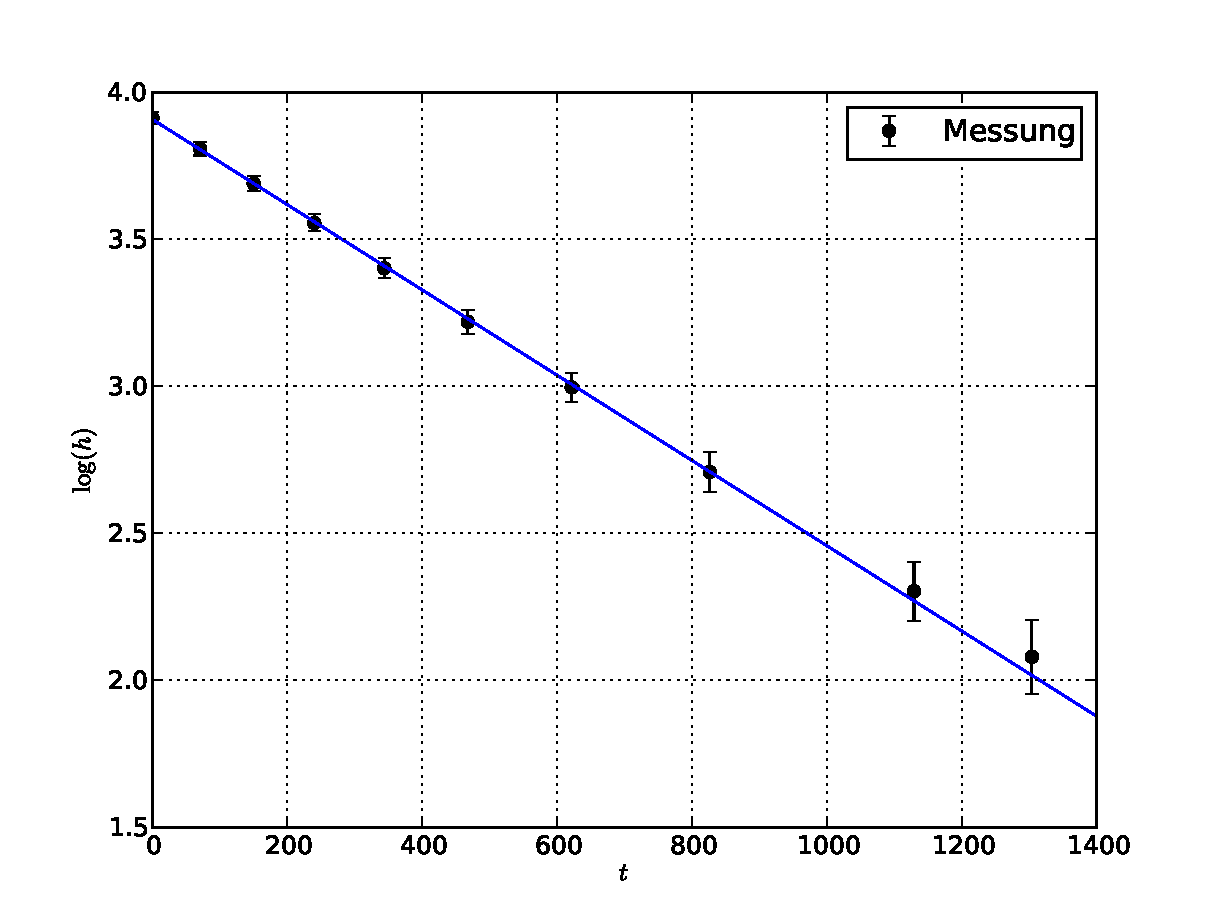
\includegraphics[scale=0.70]{Plot_Aufg2b}
%\end{center}
%\caption{Auslauf halblogarithmisch aufgetragen}
%\end{figure}
